\documentclass[a6paper,10pt]{article}
%\usepackage[T1]{fontenc}
\usepackage[british]{babel}
\usepackage[utf8]{inputenc}
\usepackage{float, graphicx,amsmath,amsfonts,cite,enumerate,tabularx}
\usepackage[final]{pdfpages}
\usepackage{wrapfig}
\usepackage[margin=0.3in]{geometry}
\usepackage{../sidspaltHack}
\usepackage{../digital}
\usepackage{ulem}


\setlength{\oddsidemargin}{-0.37in}
\setlength{\textwidth}{215pt}

\pagestyle{empty}

\begin{document}
\nysida{15}{20.1}
\noindent
\chaptertitle{$\Sigma\sigma$}{Visor vi minns}
\vspace{10pt}

\noindent
\small
På denna sida börjar sångbokens nyaste kapitel: Sigma! Målet med att införa ett kapitel som detta är att försöka \textit{summera} det gångna året på Fysiksektionen som det sett ut, eller snarare hörts ut, under gasquer, banquetter, spex eller övriga tillställningar. 

Häri finner du ett litet axplock av de sångbladstexter, gyckel och spextexter som lyckats fånga upp. Detta innebär förstås att jag missat flertalet fantastiska alster, men jag hoppas att det ändå delvis  kan återspegla året.

Givetvis påverkas sångkulturen av att sektionens verksamhet varit nedstängt under en väsentlig del av året, men även det har gett upphov till unika minnen så som sektionens första digitala tentagasque.

Vill du få med ett gyckel/en sångtext/en fin visa till nästa års summering? Tveka inte då att tipsa mig och/eller 2021 års sångboksansvariga och framför din åsikt! Många av texterna du finner här är med tack vare ivriga tips och hjälp från andra fysiker (ingen nämnd, ingen glömd). 

Jag önskar er mycket sångglädje! 
\auth{Evelina Stenseth \\Profilansvarig 2020}
\nysida{15}{20.1}
\setlength{\oddsidemargin}{-0.47in}

\begin{center}
\huge \textit{2019/2020}
\end{center}

\begin{center}
\songtitle{$\sigma20.1$}{Brev från nØllan}
\mel{Brev från Kolonien} 
\end{center}
\begin{lyrics}
\small Hejsan FRum, hejsan Styret,\\
här är brev från nØllepyret.\\
Vi har kul i Konsulatet,\\
vi står tjugoåtta schlemmiga nØllan i en
\vspace{5pt}\\
vidsträckt kö till mikrougnar,\\
nØllan väsnas, för vi hungrar.\\
Stackars fysiker som står bredvid oss,\\
de dränker bäst sin sorg med en stor flaska rom.
\vspace{5pt}\\
Vi har roligt, vill jag lova,\\
bara plugga, aldrig sova.\\
Och när tenta-P, äntligen är slut,\\
ja då vill jag gasqua och få mig en redig sup.
\vspace{5pt}\\
I Konsulatet, finns det snapsglas.\\
Ut i skogen finns det lustgas,\\
som man köper av en kul typ,\\
till ockerpriser, så nu är min plånbok tom, typ.
\vspace{5pt}\\
En bakfylla, jag sent glömmer.\\
In på toan, magen tömmer\\
ut sitt innehåll, utan förbehåll,\\
svär att jag aldrig igen ska dricka alkohol.
\nysida{15}{20.1}
\setlength{\oddsidemargin}{-0.47in}
\noindent
Nu har jag snart, slut på pengar,\\
till den 25:e, jag ivrigt längtar.\\
Och när CSN har betalats ut,\\
ja då bränner jag drygt hälften på kurslitteratur!
\vspace{5pt}\\
Jag fick hål i, mina tänder,\\
godisskåpet, sånt som händer...\\
Min diet består mest av Billys\\
och om jag tröttnar finns det snabbnudlar \\ från Willy’s.
\vspace{5pt}\\
I Konsulatet, är alla snälla,\\
jag ser inga skäl att gnälla.\\
Tack till Styret, nämnderna och allt\\
och särskilt fkm* som höjer min promillehalt!
\end{lyrics}
\auth{Alex Hamben, F-19 \\Ettans fest 2019}



\nysida{15}{20.2}
\setlength{\oddsidemargin}{-0.47in}

\begin{center}
\songtitle{$\sigma20.2$}{van der Waals}
\mel{Wondervall} 
\end{center}
\begin{lyrics}
\small Kvasistatisk, isoterm, reversibel, adiabat,\\
kontinuerligt i jämvikt, ger approximativt resultat.\\
Ofta antar vi ideal gas,\\
men räcker inte det, \\
vad gör man då?
\vspace{5pt}\\
\textit{P} plus \\
\textit{a} gånger \textit{N} över \textit{V} i parantes kvadrat\\
gånger \\
\textit{V} minus \textit{Nb} ska va lika med \textit{NkT}.\\
Om man kan räkna van der Waals\\
kommer tentan gå bra,\\
hoppas jag...
\vspace{5pt}\\
Partikeltätheten är hög och trycket är mäktigt\\
systemets temperatur är otillräcklig.\\
Det finns många fall när man\\
behöver räkna på dig,\\
men jag vet ej hur.
\vspace{5pt}\\
För \textit{PV}… \\
Är ungefär lika med \textit{NkT},\\
för en ideal gas.\\
men inte van der Waals!
\end{lyrics}
\auth{Felix Bengtsson, Alex Hamben \\ \& Marve Grönblad Vesterinen, F-19 \\Tentagasque 1 2019 - Gasque för fulla segel!}

\nysida{15}{20.3}
\setlength{\oddsidemargin}{-0.47in}

\begin{center}
\songtitle{$\sigma20.3$}{Potatiskanon}
\mel{Punschkanon (gökvisa)} 
\end{center}
\begin{lyrics}
\textit{"Herrar":}
\vspace{3pt}\\
$\|$: Potato, potato, potato, all kinds of :$\|$
\vspace{5pt}\\
\textit{"Damer":}
\vspace{3pt}\\
When we have potatoes\\
what with them can we do?\\
Boil ’em, mash’em, stick ’em in a stew.
\vspace{5pt}\\
$\|$: Potatoes! Potatoes! Even more more potatoes  :$\|$
\end{lyrics}
\auth{Frida Grönberg \& Rebecca Remling, F-19 \\Tentagasque 2 2020 - Sagan om Kons}

\vspace{20pt}
\begin{figure}[h!]
\begin{center}
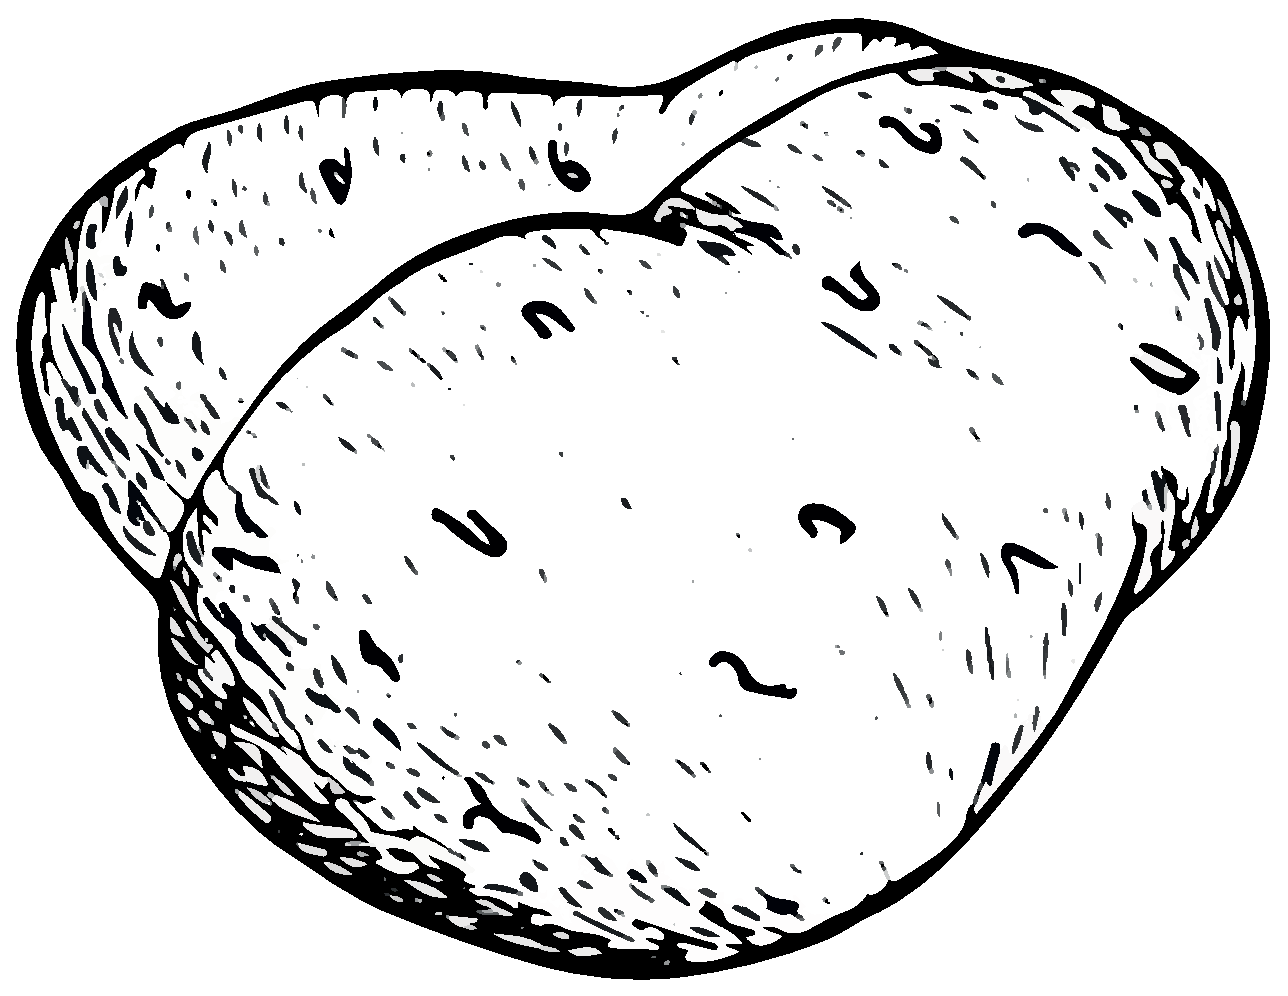
\includegraphics[width=150pt]{potatiskanon}
\end{center}
\end{figure}

\nysida{15}{20.4}
\setlength{\oddsidemargin}{-0.47in}

\begin{center}
\songtitle{$\sigma20.4$}{Sjörövar-$\pi$}
\mel{Sjörövarfabbe} 
\end{center}
\begin{lyrics}
\small 3 komma 14 ett fem ni',\\
Börjar den långa följden av $\pi$.\\
Dess decimaler blir inte $\phi$,\\
detta är en sång om $\pi$!
\vspace{5pt}\\
2 6 5 35 åttini',\\
så fortsätter följden av $\pi$.\\
Vi vet hur man beräknar $\pi$,\\
nyttja lite trolleri.
\vspace{5pt}\\
Ta en cirkel och mät runt den,\\
dra ett streck tvärs över ringen,\\
dela dessa så får du nåntin’\\
så kan du beräkna $\pi$!
\vspace{5pt}\\
Men då,\\
vad står på?\\
Decimalerna blir bara mera små.\\
Oj då,\\
vad står på?\\
Oj oj oj, oj oj oj,\\
oj, oj, oj, oj, oj, oj, oj, oj!
\vspace{5pt}\\
Det är nåt man måste förstå,\\
även om siffrorna inte är få,\\
minskar dess värde ju fler man får,\\
därför estimeras $\pi$ 
\vspace{5pt}\\
\textit{Skrik:} “till 3!”
\end{lyrics}
\auth{Nicole Hedblom F-17 \& Björn Magnusson \\Tentagasque 4 2020 - TGZoom}

\nysida{15}{20.5}
\setlength{\oddsidemargin}{-0.47in}

\begin{center}
\songtitle{$\sigma20.5$}{Numme, numme, hej!}
\mel{Dragostea din tei} 
\end{center}
\begin{lyrics}
\small $\|$: Maiahi-Maiaho, Maiaha-maiahaha :$\|$
\vspace{5pt}\\
Hallå? Salut!\\
Har ni hört om, en kurs?\\
Där man kan\\
lösa allting, numeriskt, på en dator.
\vspace{5pt}\\
Euler framåt,\\
numme, numme, hej!\\
Numme, numme, hej!\\
Numme numme, numme, yay!\\
Datorn räknar ut allting åt dig\\
så länge algoritmen sköter sig.
\vspace{5pt}\\
Euler bakåt,\\
numme, numme, hej!\\
Numme, numme, hej!\\
Numme numme numme, yay!\\
Diskret integration hjälper dig\\
när trapetsmetoden sköter sig.
\vspace{5pt}\\
Newton Raphson\\
numme, numme, hej!\\
Numme, numme, hej!\\
Numme numme numme, yay!\\
Fixpunkts metoden kan hjälpa dig\\
När \textit{x} löses ut implicit-yay!
\vspace{5pt}\\
Runge Kutta,\\
numme, numme, hej!\\
Numme, numme, hej!\\
Numme numme numme, yay!
\nysida{15}{20.5}
\setlength{\oddsidemargin}{-0.47in}
\noindent
\textit{Omstart:}
\vspace{3pt}\\
\textit{n} = 1\\
While true:\\
\indent
    \textit{n} = \textit{n} + 1\\
    \indent \textit{n}:te + "gradspolynom-\\
    \indent interpolation\\
    \indent interpolation\\
    \indent interpolatiio-o-on”\\
    \indent If \textit{många räcker upp handen} or $n>4$:\\
    \indent \indent break\\
    \indent end\\
end
\end{lyrics}
\auth{William Laius Lundgren\\ \& Gustav von Knorring, F-18\\Tentagasque 4 2020 - TGZoom}

\end{document}